\section{Marks Module}

\subsection{Problem Summary}

\hspace{0.35cm} Several exams are conducted in the course using Bodhitree platform or using traditional methods. The marks obtained by the students in the exams conducted in the course must be maintained and displayed to the students. The marks module provides functionality to upload the students marks on Bodhitree and each student can view his marks by logging into his Bodhitree account.

\subsection{Specifications}

\hspace{0.35cm} Several specification were provided on the instructors as well as the students side to ensure optimum usability.

\subsubsection*{Instructor Specifications:}

\begin{enumerate}
	\item The instructor can upload a CSV file containing the marks of the students in each of the exams that were conducted.
	\item The first line of the CSV file must be the names of the exams conducted. For example, Quiz1, Quiz2, Endsem.
	\item The second line of the CSV file must be the maximum marks that can be obtained in the quiz.
	\item The lines that follow must contain the username of the student as registered in Bodhitree followed by his marks in each of the exams.
	\item A sample is given below:
	
	\begin{center}
	\def\arraystretch{1.5}
	\begin{tabular}{|c|c|c|c|c|}
	\hline \textit{EXAM TYPE} & Q1 & Midsem & Q2 & Endsem \\ 
	\hline \textit{MAX MARKS} & 20 & 30 & 20 & 30 \\ 
	\hline stud1 & 12 & 22 & 14 & 26 \\
	\hline stud2 & 10 & 12 & 4 & 16 \\
	\hline stud3 & 0 & 23 & 10 & 28 \\
	\hline 
	\end{tabular} 
	\\ 	\vspace{0.2in} \textit{Table 1}: Format for uploading the students marks
	\end{center}
	
\end{enumerate}

\subsubsection*{Student Specifications:}

\begin{enumerate}
	\item Student log's into his Bodhitree account and can see his marks after clicking on the Marks tab on the course page.
	\item The marks must in a tabular format, with the first row showing the exams that took place in the course.
	\item The second row of the table consists of the corresponding marks scored by the student in each of those exams.
	\item The student can view only his marks, no other student's marks should be visible to him.
\end{enumerate}

\subsection{System Design}

The following functionalities were designed to complete the marks module:

\subsubsection*{CSV file upload and storing the marks:}

\begin{enumerate}
	\item The instructor uploads a CSV file which contains the marks of the student in the format as shown in table 1.
	\item The system parses the CSV file and stores the marks in the database in the following manner:
	\begin{enumerate}
		\item The marks headers are stored in the table \textbf{marksheader} having 5 fields: \textit{id, course id, exam type} and \textit{maximum marks}.
		\item The actual marks obtained by the students are stored in another table \textbf{mark} which has the following fields: \textit{id, marksheader id, student id, marks}.
		\item The marksheader id of the mark table is a foreign key to the marksheader table.
		\item Snapshots of the tables are shown below:
	\end{enumerate}
\end{enumerate}
\newpage		
	\begin{figure}[h]
	\centering
	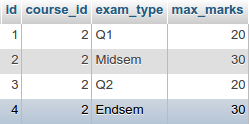
\includegraphics[width=0.4\linewidth]{./media/MarksHeader}
	\caption{Database table of the marks header}
	\label{fig:MarksHeader}
	\end{figure}
	\begin{figure}[h]
	\centering
	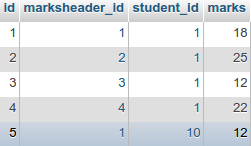
\includegraphics[width=0.4\linewidth]{./media/mark}
	\caption{Database table of students marks}
	\label{fig:mark}
	\end{figure}

\subsubsection*{Displaying student's marks:}
\begin{enumerate}
	\item The user id of the currenty logged in user and the current course id are the fields that are taken into consideration. They are then used to fetch the data that follows.
	\item Each exam and the corresponding maximum marks are fetched from the marks header table.
	\item Then the marks obtained by the student in each of these exams are fetched.
\end{enumerate}

\subsubsection*{Handling authentication:}
\begin{enumerate}
	\item If and only if the current logged in user is an Instructor or a Content Developer, then he can view the marks upload page.
	\item The students cannot view the marks of other students.
	\item A user who has not logged in cannot view any interface of the marks module.
\end{enumerate}

\newpage

\subsection*{Screenshots of the system:}

\begin{figure}[h]
\centering
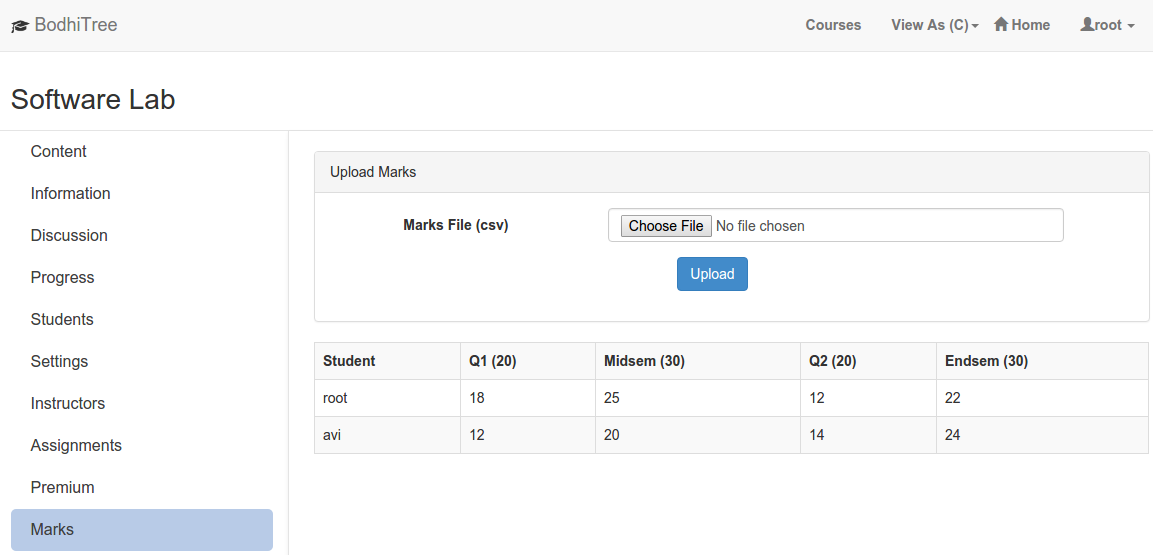
\includegraphics[width=0.95\linewidth]{./media/CDmarks}
\caption{Instructor's interface for uploading the CSV file}
\label{fig:CDmarks}
\end{figure}
\begin{figure}[h]
\centering
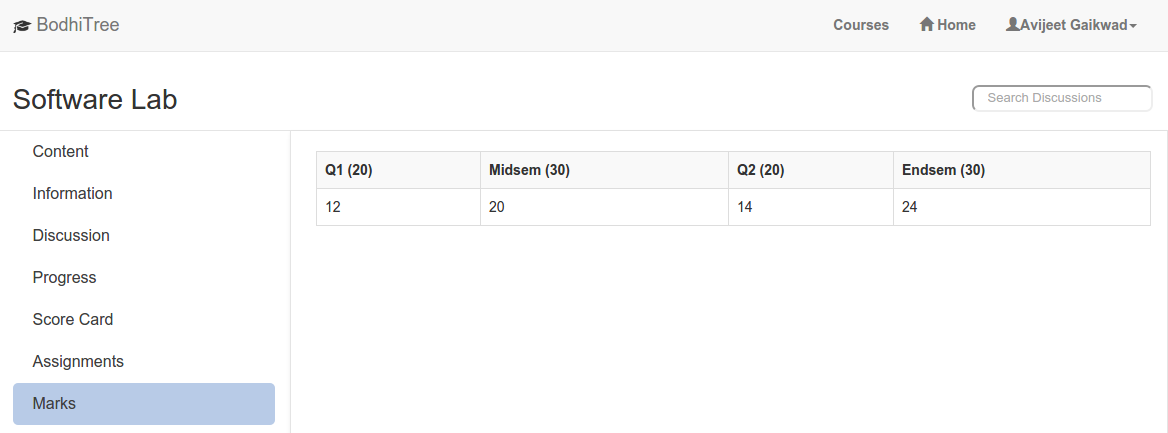
\includegraphics[width=0.95\linewidth]{./media/Smarks}
\caption{Student's interface for viewing his/her marks}
\label{fig:Smarks}
\end{figure}

%\subsection{Future Work}